
\begin{center}
\thispagestyle{empty}


\vspace{.5cm}

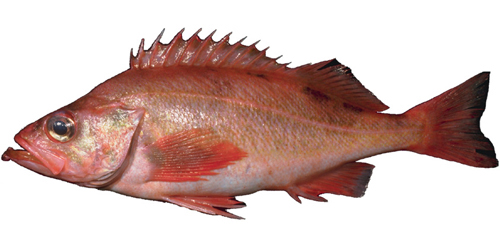
\includegraphics{Sebastes_alutus}~\\[0.5cm]
%\pdftooltip{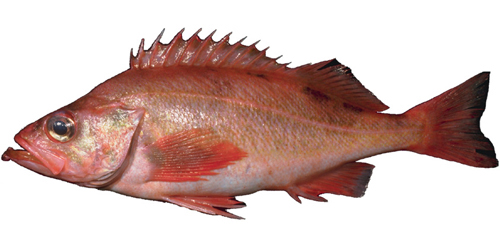
\includegraphics{Sebastes_alutus}}{This is a fish.}



Chantel R. Wetzel\textsuperscript{1}\\
Lee Cronin-Fine\textsuperscript{2}\\
Kelli F. Johnson\textsuperscript{1,2}\\

\vspace{.5cm}

\small
\textsuperscript{1}Northwest Fisheries Science Center, U.S. Department of Commerce, National Oceanic and Atmospheric Administration, National Marine Fisheries Service, 2725 Montlake Boulevard East, Seattle, Washington 98112\\

\vspace{.3cm}

\textsuperscript{2}University of Washington, School of Aquatic and Fishery Sciences\\





\vspace{1cm}

\vfill
DRAFT SAFE\\
Disclaimer: This information is distributed solely for the purpose of pre-dissemination
peer review under applicable information quality guidelines. It has not been formally
disseminated by NOAA Fisheries. It does not represent and should not be construed to
represent any agency determination or policy. 



\vspace{.3cm}
%Bottom of the page
%{\large \today}

\newpage

\vspace{3cm}

Please cite as:\\

Wetzel, C.R., Cronin-Fine, L., and Johnson, K.F. 2017. Status of Pacific ocean perch (\textit{Sebastes alutus}) along the US west coast in 2017. Pacific Fishery Managment Council, 7700 Ambassador Place NE, Suite 200, Portland, OR 97220. 

\vspace{3cm}

\maketitle






\pagenumbering{roman}
\setcounter{page}{1}
\end{center}


